\chapter{Biologia da Conservação}\label{ch:b3:conservation-biology}

Em 1813 Audubon viu um bando de pombos-passageiros passar sobre o
Kentucky por três dias, escurecendo o céu; eram talvez cinco bilhões
deles, um quarto de todas as aves da América do Norte. Em 1º~de setembro
de 1914 o último deles, uma fêmea chamada Martha, morreu no zoológico de
Cincinnati. A espécie não era rara quando seu declínio começou; ela foi
colhida a vagões de trem, suas florestas foram cortadas, e uma ave que só
se reproduzia em colônias imensas não conseguiu mais se reproduzir depois
que as colônias rarearam abaixo de um tamanho que ninguém mediu. Em 1995
o kakapo, um papagaio noturno e não voador da Nova Zelândia, estava
reduzido a cinquenta e uma aves; cada uma delas foi desde então nomeada,
pesada, equipada com um transmissor e, no momento certo, servida com uma
refeição suplementar, e hoje são duzentas e cinquenta. No mesmo ano trinta
e um lobos-cinzentos foram soltos em Yellowstone, setenta anos depois de a
última alcateia nativa ter sido abatida; em duas décadas os wapitis haviam
se deslocado, os salgueiros tinham voltado ao longo dos rios, e os castores
com eles. A biologia da conservação é a aplicação da genética de
populações, da ecologia e do comportamento deste livro a uma única
pergunta prática --- como impedir que as espécies desapareçam --- e sua
aritmética é a aritmética dos números pequenos.

\section{Por que as populações pequenas morrem}

\begin{definition}[Os riscos da pequenez]\label{def:b3:conservation-biology:small}
\index{estocasticidade demográfica}\index{estocasticidade ambiental}\index{efeito Allee}\index{vórtice de extinção}\index{população mínima viável}
Uma população grande declina quando sua \omterm{prop:b3:stem-cells:gompertz}{taxa de mortalidade} excede a de
natalidade; uma pequena pode sumir sem qualquer mudança em nenhuma das
duas. A \emph{estocasticidade demográfica} é a chance de que, entre uns
poucos indivíduos, morram mais do que nascem, ou de que todos os
sobreviventes sejam machos: ela importa abaixo de algumas dezenas. A
\emph{estocasticidade ambiental} --- um inverno ruim, uma seca, uma
doença --- atinge todos os indivíduos de uma só vez, e uma população de
algumas centenas que uma grande atravessaria sem problema pode ser
varrida; as \emph{catástrofes} são sua cauda. O \emph{efeito Allee} faz a
taxa de crescimento per capita cair em densidade baixa --- não se acham
parceiros, os reprodutores coloniais não conseguem nidificar, os rebanhos
não conseguem defender seus filhotes, os bandos do pombo-passageiro não
conseguiam saturar os predadores que levavam seus filhotes ---, de modo
que abaixo de uma densidade-limiar a população declina rumo a zero por
conta própria. E abaixo de algumas centenas, os processos genéticos da
próxima seção reduzem a aptidão geração após geração. Uns alimentam os
outros: uma população menor perde variação, fica menos fértil, encolhe,
tem mais chance de ser atingida pelo acaso e perde mais --- o
\emph{vórtice de extinção} (Gilpin e Soulé, 1986). Uma \emph{população
mínima viável} é o tamanho acima do qual a probabilidade de extinção num
horizonte declarado (digamos, \qty{5}{\%} num século) é aceitável; ela
depende da biologia da espécie e de quão variável é seu ambiente, e em
geral está na casa dos milhares.
\end{definition}

\begin{omfigure}
\begin{tikzpicture}[every node/.style={font=\scriptsize}, >=stealth]
  \node[draw, thick, rounded corners, fill=omThm!20, align=center] (small) at (0,0) {a população\\fica pequena};
  \node[draw, thick, rounded corners, fill=omDef!20, align=center] (drift) at (3.4,1.6) {deriva e endogamia:\\variação perdida, $F$ sobe};
  \node[draw, thick, rounded corners, fill=omDef!20, align=center] (fit) at (6.8,0) {a aptidão cai:\\menos filhotes, mais doença};
  \node[draw, thick, rounded corners, fill=omDef!20, align=center] (chance) at (3.4,-1.6) {o acaso demográfico e ambiental\\morde mais forte};
  \node[draw, thick, rounded corners, fill=omProp!25, align=center] (allee) at (9.9,0) {efeito Allee:\\taxa de crescimento negativa};
  \draw[->, very thick] (small) -- (drift); \draw[->, very thick] (drift) -- (fit); \draw[->, very thick] (fit) -- (chance); \draw[->, very thick] (chance) -- (small);
  \draw[->, thick, omProp!80!black] (fit) -- (allee); \draw[->, thick, omProp!80!black] (allee.south) .. controls (9.9,-3) and (0,-3.4) .. (small.south);
  \node[align=center, font=\tiny] at (3.4,0) {o vórtice de extinção:\\cada volta encolhe a\\população e acelera a seguinte};
  \node[left, align=right, font=\tiny] at (-1.7,1.5) {perda de hábitat, caça,\\predadores invasores,\\doença empurram a\\população para dentro};
  \draw[->, thick, gray] (-1.6,1.2) -- (small.north west);
\end{tikzpicture}

{\small O \omterm{def:b3:conservation-biology:small}{vórtice de extinção}. Um golpe externo torna uma população
pequena; a pequenez então faz perder variação, baixa a aptidão, expõe a
população ao acaso e a torna ainda menor. A tarefa da conservação é
romper a alça antes que ela se feche.}
\end{omfigure}

\begin{theorem}[Tamanho efetivo da população]\label{thm:b3:conservation-biology:ne}
\index{tamanho efetivo da população}\index{razão sexual}\index{média harmônica}\index{coeficiente de endogamia}\index{heterozigosidade}
A velocidade com que uma população perde variação e acumula endogamia é
governada não por seu tamanho censitário $N$, mas por seu \emph{tamanho
efetivo} $N_{e}$: o tamanho de uma população ideal --- constante, com
acasalamento aleatório, \omterm{thm:b3:conservation-biology:ne}{razão sexual} igual e tamanhos de família de
Poisson --- que perderia heterozigosidade na mesma velocidade. Três
desvios do ideal o reduzem. A \omterm{thm:b3:conservation-biology:ne}{razão sexual} desigual, com $N_{m}$ machos e
$N_{f}$ fêmeas reprodutores:
\[
N_{e} = \frac{4N_{m}N_{f}}{N_{m} + N_{f}} ;
\]
um macho e cem fêmeas dão $N_{e} \approx 4$. O tamanho flutuante ao longo
de $t$ gerações: $N_{e}$ é a \emph{\omterm{thm:b3:conservation-biology:ne}{média harmônica}} dos tamanhos das
gerações, $1/N_{e} = (1/t)\sum 1/N_{i}$, dominada pelo menor --- uma
população de mil que uma vez passou por dez tem $N_{e}$ perto de cem
nesse intervalo. E a variância no tamanho da família acima da de Poisson
o reduz ainda mais. Numa população de tamanho efetivo $N_{e}$ o
\emph{\omterm{thm:b3:conservation-biology:ne}{coeficiente de endogamia}} $F$ --- a probabilidade de que os dois
alelos de um locus num indivíduo sejam cópias de um mesmo alelo ancestral
--- sobe $1/2N_{e}$ por geração,
\[
F_{t} = 1 - \Bigl(1 - \frac{1}{2N_{e}}\Bigr)^{t} \approx \frac{t}{2N_{e}},
\qquad H_{t} = H_{0}\Bigl(1 - \frac{1}{2N_{e}}\Bigr)^{t} ,
\]
e a \emph{heterozigosidade} $H$ decai na mesma velocidade. A regra
prática de Franklin, ``50/500'': $N_{e} \ge 50$ mantém a endogamia abaixo
de \qty{1}{\%} por geração, a taxa que os criadores de animais toleram;
$N_{e} \ge
500$ permite que a mutação reponha a variação que a deriva
retira. Como $N_{e}$ é tipicamente um décimo do tamanho censitário, a
regra pede populações de quinhentos a cinco mil.
\end{theorem}
\begin{proof}
Dois gametas sorteados ao acaso da população são cópias do mesmo alelo
parental com probabilidade $1/2N$ na população ideal, que é o incremento
de $F$; a heterozigosidade é $1 - F$ reescalado, de modo que cada geração
a multiplica por $(1 - 1/2N_{e})$, dando o decaimento exponencial e, para
$t \ll N_{e}$, a subida linear de $F$. \omterm{thm:b3:conservation-biology:ne}{Razão sexual}: metade dos genes vem
de cada sexo, de modo que a chance de dois gametas compartilharem um
alelo parental é $\tfrac{1}{4}\cdot\tfrac{1}{2N_{m}} +
\tfrac{1}{4}\cdot\tfrac{1}{2N_{f}}$ (um quarto dos pares são ambos
paternos, e um quarto ambos maternos); igualando isso a $1/2N_{e}$
obtém-se $1/N_{e} = 1/(4N_{m}) + 1/(4N_{f})$, a fórmula. Flutuação: a
heterozigosidade após $t$ gerações é $H_{0}\prod(1 - 1/2N_{i})
\approx H_{0}\exp(-\sum 1/2N_{i})$, igual a $H_{0}\exp(-t/2N_{e})$ quando
$1/N_{e}$ é a média dos $1/N_{i}$. A endogamia baixa a aptidão porque
expõe alelos recessivos deletérios em homozigose --- a \emph{depressão
endogâmica}, uma queda de alguns por cento na sobrevivência ou na
fecundidade a cada \qty{10}{\%} de $F$ na maioria das espécies
exogâmicas.
\end{proof}

\begin{omfigure}
\begin{tikzpicture}
\begin{axis}[
  width=0.46\linewidth, height=5.2cm,
  axis x line=bottom, axis y line=left,
  xmin=0, xmax=1, ymin=0, ymax=1.05,
  xlabel={fração dos reprodutores que são machos}, ylabel={$N_{e}/N$},
  xlabel style={font=\small, at={(axis description cs:0.5,-0.12)}, anchor=north}, ylabel style={font=\small},
  tick label style={font=\small}, xtick={0,0.1,0.5,0.9,1}, ytick={0.36,1},
  clip=false,
]
\addplot[very thick, omDef, domain=0.005:0.995, samples=100] {4*x*(1-x)};
\draw[dashed, gray] (axis cs:0.1,0) -- (axis cs:0.1,0.36) -- (axis cs:0,0.36);
\node[font=\scriptsize, omDef, anchor=south] at (axis cs:0.5,1.0) {sexos iguais: $N_{e} = N$};
\node[font=\scriptsize, anchor=west, align=left] at (axis cs:0.12,0.2) {um macho em dez\\se reproduz: $N_{e} = 0.36N$};
\end{axis}
\begin{axis}[
  at={(0.5\linewidth,0)}, anchor=south west,
  width=0.46\linewidth, height=5.2cm,
  axis x line=bottom, axis y line=left,
  xmin=0, xmax=100, ymin=0, ymax=1.05,
  xlabel={gerações}, ylabel={heterozigosidade $H_{t}/H_{0}$},
  xlabel style={font=\small, at={(axis description cs:0.5,-0.12)}, anchor=north}, ylabel style={font=\small},
  tick label style={font=\small}, xtick={0,25,50,75,100}, ytick={0.37,0.6,0.9,1},
  yticklabels={0.37,0.6,0.9,1},
  clip=false,
]
\addplot[very thick, omThm, domain=0:100, samples=60] {(1-1/20)^x};
\addplot[very thick, omMeth!70!black, domain=0:100, samples=60] {(1-1/100)^x};
\addplot[very thick, omDef, domain=0:100, samples=60] {(1-1/1000)^x};
\node[font=\scriptsize, omThm, anchor=north west] at (axis cs:12,0.55) {$N_{e} = 10$};
\node[font=\scriptsize, omMeth!70!black, anchor=south west] at (axis cs:50,0.62) {$N_{e} = 50$};
\node[font=\scriptsize, omDef, anchor=south west] at (axis cs:60,0.95) {$N_{e} = 500$};
\end{axis}
\end{tikzpicture}

{\small À esquerda: como uma \omterm{thm:b3:conservation-biology:ne}{razão sexual} desequilibrada encolhe o
tamanho efetivo --- uma espécie de haréns com um décimo dos machos se
reproduzindo tem um $N_{e}$ igual a um terço de seu censo. À direita: a
heterozigosidade decaindo por $(1 - 1/2N_{e})$ a cada geração --- uma
população de dez perde a maior parte de sua variação num século, e uma de
quinhentas quase nada.}
\end{omfigure}

\begin{proof}[Evidência]
A pantera-da-flórida, reduzida a uns vinte e cinco animais nos anos 1990,
apresentava caudas tortas, testículos que não desciam, defeitos cardíacos
e espermatozoides dos quais \qty{90}{\%} eram anormais --- a depressão
endogâmica tornada visível; oito fêmeas introduzidas do Texas em 1995 (o
\emph{resgate genético}) triplicaram a população e os defeitos recuaram.
Os lobos da Ilha Royale, fundados por um casal em 1949 e isolados,
declinaram a dois indivíduos grosseiramente endogâmicos até 2018, com
deformidades da coluna na maioria dos esqueletos examinados. A
galinha-da-pradaria-grande de Illinois caiu de milhares para cinquenta, e
sua taxa de eclosão dos ovos de \qty{93}{\%} para \qty{56}{\%},
recuperando-se depois que aves foram trazidas de outros estados. Peles de
museu e DNA antigo permitiram medir diretamente a perda de
heterozigosidade em relação à população anterior ao declínio em cada
caso.
\end{proof}

\begin{omfigure}
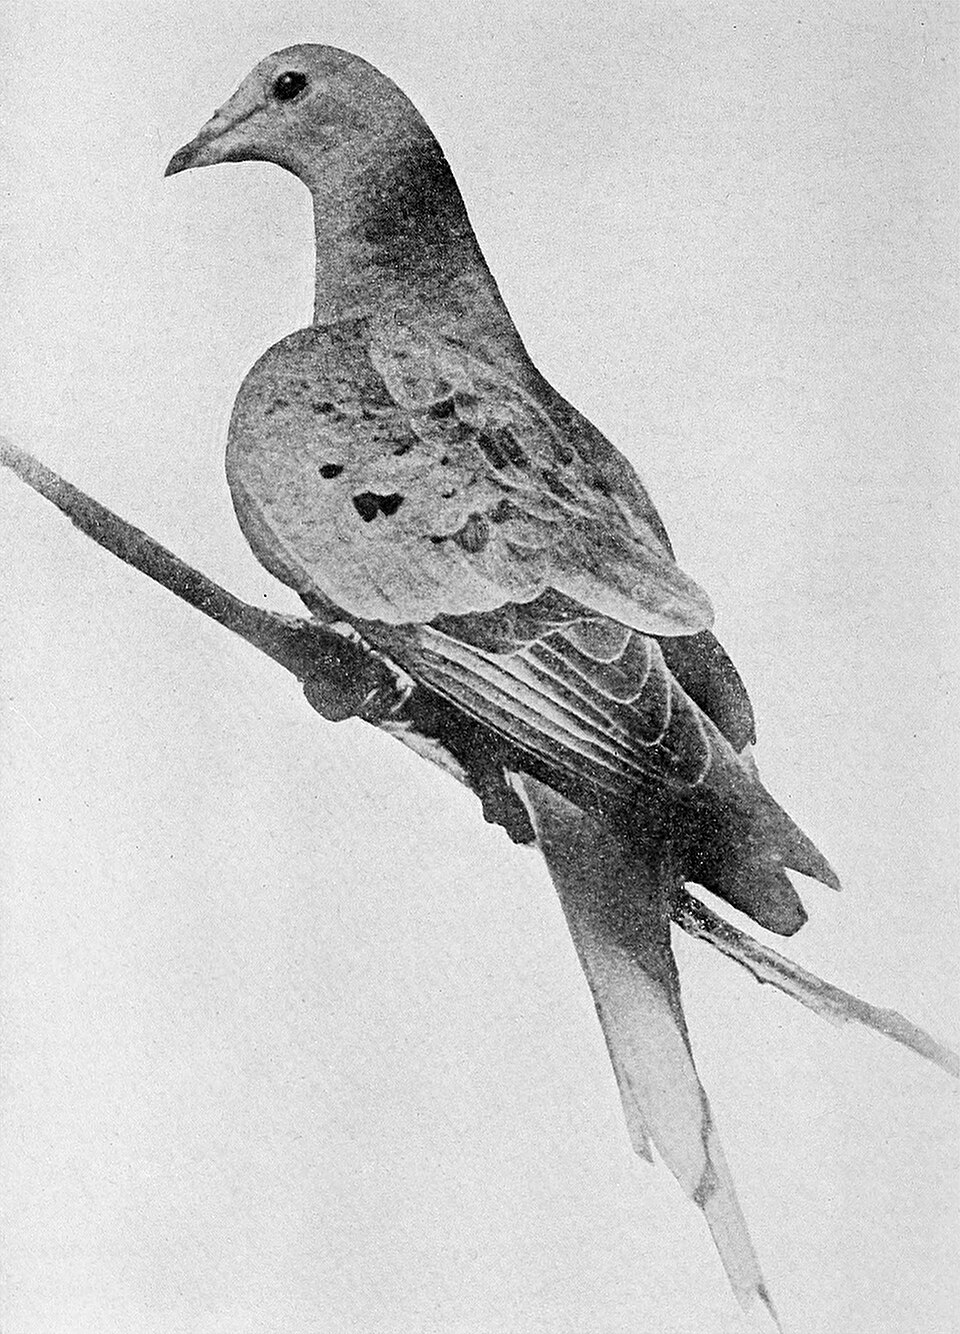
\includegraphics[width=0.4\linewidth]{images/book5/martha.jpg}\hspace{0.04\linewidth}
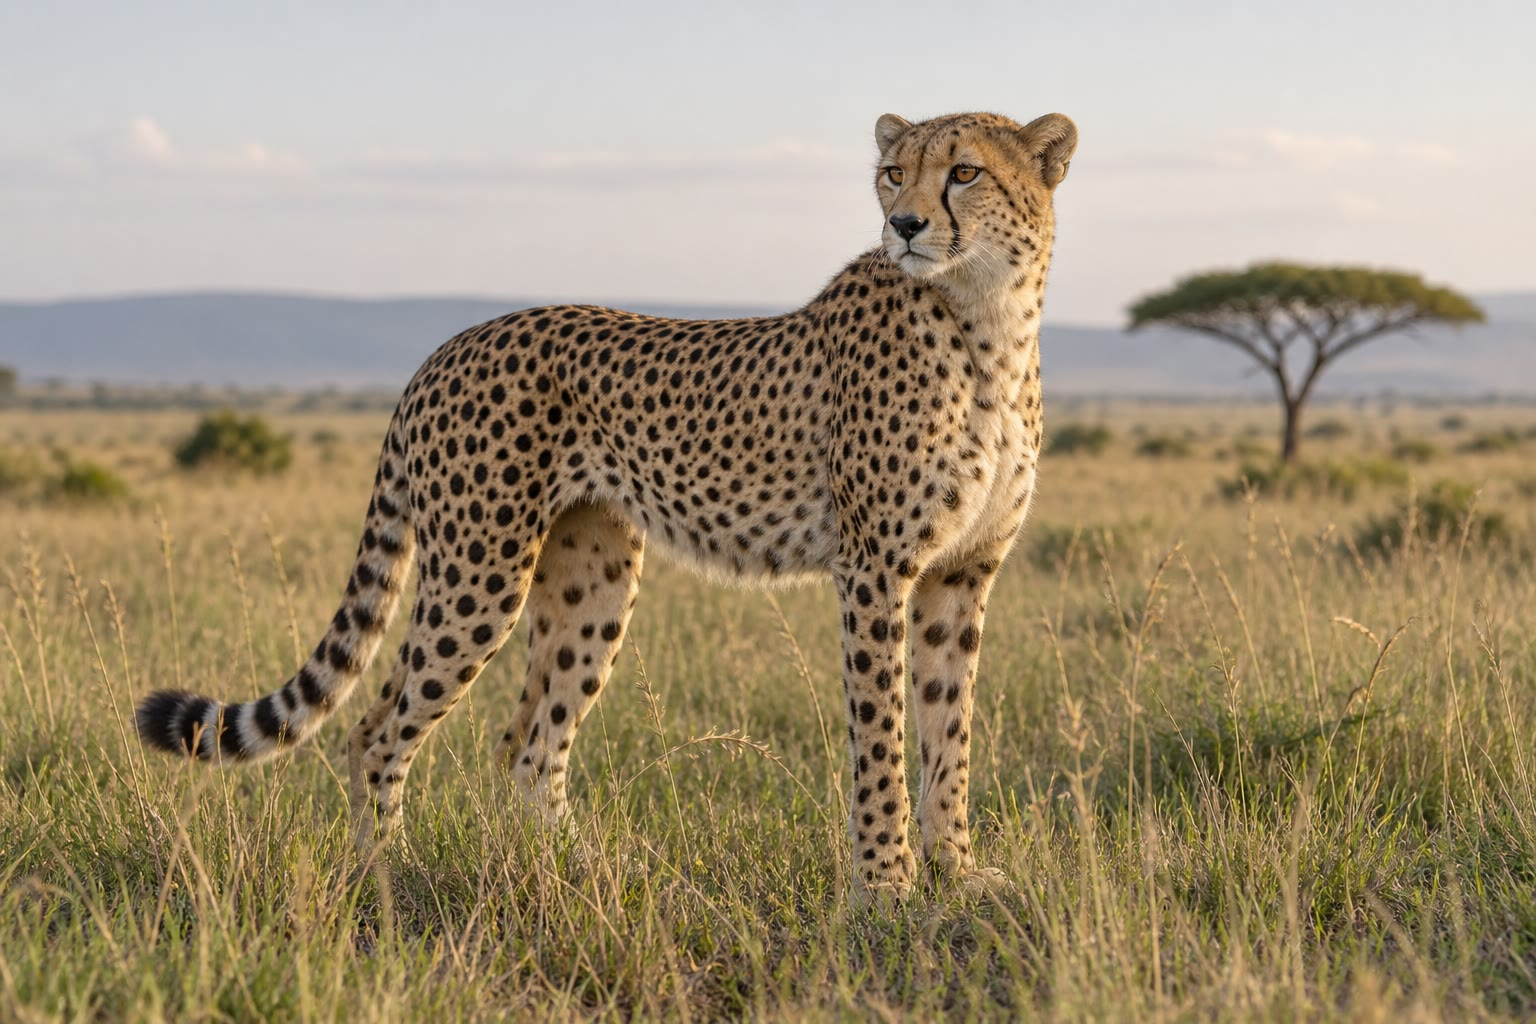
\includegraphics[width=0.52\linewidth]{images/book5/ai/b5-27-cheetah.jpg}

{\small À esquerda: Martha, o último pombo-passageiro, fotografada no
zoológico de Cincinnati em 1912; a espécie tinha sido de bilhões dentro
da memória de quem vivia (fotografia de Enno Meyer, domínio público). À
direita: um guepardo --- uma espécie que passou por um gargalo uns dez
mil anos atrás e cujos indivíduos são tão parecidos que enxertos de pele
entre animais não aparentados não são rejeitados.}
\end{omfigure}

\section{Hábitat: quanto, e com que forma}

\begin{proposition}[Espécies e área]\label{prop:b3:conservation-biology:area}
\index{relação espécies--área}\index{fragmentação de hábitat}\index{biogeografia de ilhas}\index{corredor}\index{debate SLOSS}\index{efeito de borda}
Entre ilhas, e entre fragmentos de hábitat que se comportam como ilhas, o
número de espécies $S$ sobe com a área $A$ como uma lei de potência,
\[
S = c\,A^{z}, \qquad z \approx 0.15\text{--}0.35,
\]
a \emph{\omterm{prop:b3:conservation-biology:area}{relação espécies--área}} (Arrhenius, 1921; a \omterm{prop:b3:conservation-biology:area}{biogeografia de ilhas}
de MacArthur e Wilson, 1967, a explicou como um equilíbrio entre
imigração e extinção, sendo a extinção mais rápida nas ilhas pequenas).
Com $z = 0.25$, perder \qty{90}{\%} da área de um hábitat acaba por
perder $1 - 0.1^{0.25} = \qty{44}{\%}$ de suas espécies; perder metade
perde \qty{16}{\%}. A perda não é imediata --- uma \emph{dívida de
extinção} é paga ao longo de décadas, à medida que populações pequenas
demais para seus fragmentos definham --- e a \emph{fragmentação} de uma
área fixa em pedaços acrescenta perdas próprias: cada fragmento abriga uma
população menor, os \emph{\omterm{prop:b3:conservation-biology:area}{efeitos de borda}} (vento, calor, predadores,
ervas daninhas) penetram centenas de metros floresta adentro, e as
espécies que precisam do interior perdem mais do que a área explica. Se
uma única reserva grande ou várias pequenas de mesma área total salvam
mais espécies (o debate \emph{SLOSS}) depende das espécies: a grande
abriga populações maiores e hábitat de interior, e as pequenas espalham o
risco de uma catástrofe e amostram mais tipos de hábitat. Os
\emph{corredores} que conectam fragmentos deixam indivíduos e genes se
moverem entre eles, transformando populações isoladas numa metapopulação
cujas partes podem ser recolonizadas após uma extinção local e resgatadas
da endogamia --- e é por isso que a terra entre as reservas virou uma
preocupação tanto quanto as próprias reservas.
\end{proposition}
\begin{proof}
A lei de potência é empírica, ajustada em eixos log--log a arquipélagos,
lagos, topos de montanha e fragmentos de floresta pelo mundo todo; o
valor de $z$ é menor para pedaços de um continente (a imigração mantém as
espécies presentes) e maior para ilhas verdadeiras. A perda fracionária
decorre diretamente: $S'/S = (A'/A)^{z}$. O mecanismo da \omterm{prop:b3:conservation-biology:area}{biogeografia de
ilhas} foi testado por Simberloff e Wilson (1969), que fumigaram pequenas
ilhotas de mangue na Flórida, matando todos os artrópodes, e observaram
os números de espécies voltarem a seus valores anteriores em um ano ---
um equilíbrio, com espécies diferentes das de antes: o número é fixado
pela área e pela distância, e as identidades, pelo acaso.
\end{proof}

\begin{omfigure}
\begin{tikzpicture}
\begin{loglogaxis}[
  width=0.6\linewidth, height=5.4cm,
  axis x line=bottom, axis y line=left,
  xmin=0.5, xmax=20000, ymin=5, ymax=300,
  xlabel={área (km$^2$)}, ylabel={número de espécies},
  xlabel style={font=\small, at={(axis description cs:0.5,-0.12)}, anchor=north}, ylabel style={font=\small},
  tick label style={font=\small}, xtick={1,10,100,1000,10000}, xticklabels={1,10,100,1000,10000}, ytick={10,30,100,300}, yticklabels={10,30,100,300},
  clip=false,
]
\addplot[very thick, omDef, domain=0.5:20000, samples=40] {20*x^0.25};
\addplot[only marks, mark=*, mark size=1.8pt, omDef!70!black] coordinates {(1,22) (3,24) (10,38) (30,44) (100,66) (300,80) (1000,110) (3000,150) (10000,190)};
\draw[dashed, gray] (axis cs:10000,5) -- (axis cs:10000,200) -- (axis cs:0.5,200);
\draw[dashed, gray] (axis cs:1000,5) -- (axis cs:1000,112.5) -- (axis cs:0.5,112.5);
\node[font=\scriptsize, omDef, anchor=south west] at (axis cs:1.2,215) {$S = c\,A^{0.25}$: inclinação $z$ em eixos log};
\node[font=\scriptsize, anchor=west, align=left] at (axis cs:1200,40) {perder \qty{90}{\%} da área:\\manter $0.1^{0.25} = \qty{56}{\%}$\\das espécies};
\end{loglogaxis}
\end{tikzpicture}

{\small A lei espécies--área em eixos logarítmicos. Sua inclinação é o
expoente $z$; dela se pode ler a perda final de espécies de um hábitat
encolhido --- um décimo da floresta mantém cerca de metade das espécies,
e não o décimo que um palpite linear daria.}
\end{omfigure}

\begin{omfigure}
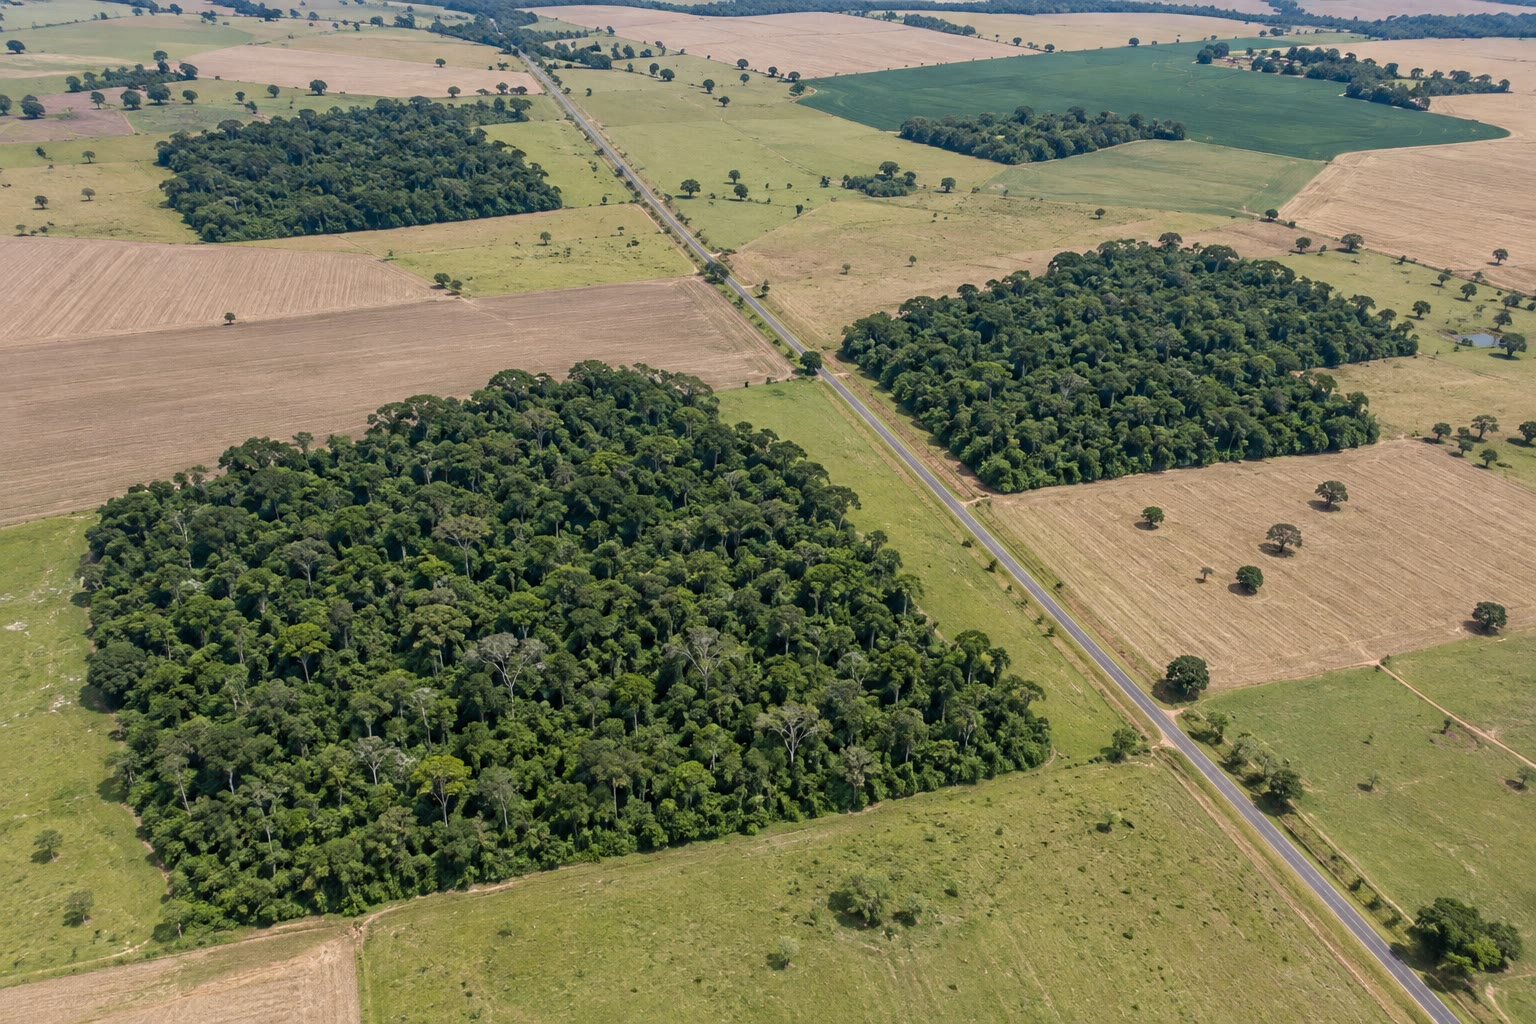
\includegraphics[width=0.6\linewidth]{images/book5/ai/b5-27-forest-fragments.jpg}

{\small Fragmentos de floresta em terras agrícolas, vistos do ar: cada
ilha abriga uma população menor que a do todo, debruada por uma faixa que
as espécies do interior não conseguem usar, e separada por campos que as
espécies florestais não conseguem atravessar.}
\end{omfigure}

\section{Prever e prevenir}

\begin{method}[Análise de viabilidade populacional]\label{met:b3:conservation-biology:pva}
\index{análise de viabilidade populacional}\index{quase extinção}
Para estimar o risco de extinção de uma população e o que o reduziria:
(1) construa um modelo de sua dinâmica --- uma matriz de sobrevivência e
fecundidade específicas por idade ou estágio, como na demografia do
volume do Ano~2, estimada a partir de indivíduos marcados ao longo de
vários anos; (2) acrescente estocasticidade --- demográfica, sorteando ao
acaso o destino de cada indivíduo, e ambiental, sorteando as taxas de
cada ano a partir de sua variância observada, com catástrofes
ocasionais; (3) acrescente dependência da densidade e o declínio genético
da endogamia onde os dados permitirem; (4) simule milhares de
trajetórias a partir do tamanho atual ao longo do horizonte de interesse
e registre a fração que cai abaixo de um limiar de \emph{\omterm{met:b3:conservation-biology:pva}{quase extinção}}
(um tamanho a partir do qual se julga impossível a recuperação); (5)
varie as entradas --- sobrevivência de adultos, sobrevivência de jovens,
área de hábitat, uma translocação de dez animais --- e veja que mudança
mais reduz o risco; é para lá que o esforço deve ir. A saída é uma
probabilidade com ampla incerteza, e não uma previsão; seu valor é
comparativo, e ela mostrou repetidamente que a sobrevivência dos adultos,
e não a fecundidade, é a alavanca nas espécies longevas, e é por isso que
as linhas de pesca matam as populações de albatrozes que põem um ovo a
cada dois anos mais depressa do que qualquer perda de ninhos conseguiria.
\end{method}

\begin{proposition}[Tempo até a extinção]\label{prop:b3:conservation-biology:time}
\index{tempo de extinção}
Para uma população que flutua porque o ambiente flutua, com taxa média de
crescimento $\bar r$ perto de zero e variância $\sigma^{2}$ na taxa anual
de crescimento, o logaritmo do tamanho populacional faz um passeio
aleatório com deriva, e o tempo esperado até a extinção a partir de um
tamanho $N$ cresce apenas com o \emph{logaritmo} de $N$ quando $\bar r < 0$ --- dobrar a população acrescenta um número fixo de anos --- e com uma
\emph{potência} de $N$ quando $\bar r > 0$, com expoente $2\bar r/\sigma^{2} - 1$; sob \omterm{def:b3:conservation-biology:small}{estocasticidade demográfica} apenas, ele cresce
\emph{exponencialmente} com $N$, de modo que uma população segura do
acaso demográfico com cem indivíduos ainda pode ser perdida para a
variância ambiental com dez mil. A consequência prática é que reduzir a
variância do crescimento de uma população --- amortecendo-a contra os
anos ruins com mais hábitat, mais sítios, uma dieta mais ampla --- pode
fazer mais por sua persistência que elevar sua média.
\end{proposition}
\admitted

\begin{omfigure}
\begin{tikzpicture}
\begin{semilogyaxis}[
  width=0.62\linewidth, height=5.4cm,
  axis x line=bottom, axis y line=left,
  xmin=0, xmax=50, ymin=1, ymax=3000,
  xlabel={anos}, ylabel={tamanho da população},
  xlabel style={font=\small, at={(axis description cs:0.5,-0.12)}, anchor=north}, ylabel style={font=\small},
  tick label style={font=\small}, xtick={0,10,20,30,40,50}, ytick={1,10,100,1000}, yticklabels={1,10,100,1000},
  clip=false,
]
\addplot[thick, omDef] coordinates {(0,200) (2,240) (4,190) (6,260) (8,300) (10,220) (12,180) (14,250) (16,330) (18,280) (20,350) (22,300) (24,260) (26,340) (28,420) (30,380) (32,450) (34,400) (36,520) (38,480) (40,560) (42,500) (44,600) (46,650) (48,610) (50,700)};
\addplot[thick, omThm] coordinates {(0,200) (2,150) (4,180) (6,120) (8,90) (10,110) (12,70) (14,50) (16,60) (18,35) (20,40) (22,25) (24,18) (26,22) (28,12) (30,8) (32,9) (34,5) (36,3) (38,2) (40,1)};
\addplot[thick, omMeth!70!black] coordinates {(0,200) (2,210) (4,170) (6,200) (8,140) (10,160) (12,120) (14,140) (16,90) (18,110) (20,80) (22,95) (24,60) (26,75) (28,50) (30,55) (32,40) (34,45) (36,30) (38,35) (40,28) (42,30) (44,22) (46,25) (48,20) (50,22)};
\draw[dashed, gray] (axis cs:0,20) -- (axis cs:50,20); \node[font=\scriptsize, gray, anchor=north east] at (axis cs:49,18) {limiar de quase extinção};
\node[font=\scriptsize, omDef, anchor=west] at (axis cs:50.5,700) {$\bar r > 0$: persiste};
\node[font=\scriptsize, omMeth!70!black, anchor=west] at (axis cs:50.5,22) {$\bar r \approx 0$: derivando para baixo};
\node[font=\scriptsize, omThm, anchor=west] at (axis cs:40.5,1.3) {$\bar r < 0$: some em 40 anos};
\end{semilogyaxis}
\end{tikzpicture}

{\small Três trajetórias simuladas a partir dos mesmos duzentos animais,
diferindo apenas na taxa média de crescimento; uma análise de viabilidade
roda milhares delas e conta quantas cruzam o limiar. A variância de ano
para ano é o que torna até o caso do meio uma aposta.}
\end{omfigure}

\begin{definition}[As ferramentas]\label{def:b3:conservation-biology:tools}
\index{Lista Vermelha da IUCN}\index{espécie invasora}\index{conservação ex situ}\index{reprodução em cativeiro}\index{reintrodução}\index{reflorestamento faunístico}\index{cascata trófica}
A \emph{Lista Vermelha da IUCN} classifica as espécies por critérios
quantitativos: um declínio de \qty{30}{\%}, \qty{50}{\%} ou \qty{80}{\%}
em dez anos ou três gerações, uma área de distribuição abaixo de
\qty{20000}{}, \qty{5000}{} ou \qty{100}{km^2}, uma população abaixo de
\qty{10000}{}, \qty{2500}{} ou \qty{250}{} indivíduos maduros, ou uma
probabilidade de extinção modelada, colocam uma espécie como Vulnerável,
Em Perigo ou Criticamente em Perigo; um quarto dos mamíferos e um oitavo
das aves se enquadram. As causas são, primeiro, a perda de hábitat;
depois, a sobre-exploração, as \emph{espécies invasoras} (predadores e
competidores levados a ilhas cujas espécies nunca os haviam encontrado:
ratos, gatos e arminhos levaram a maior parte das aves da Nova Zelândia,
e uma única espécie de cobra-arborícola-marrom, a maior parte das de
Guam), a poluição e a mudança climática. As respostas: áreas protegidas
cobrindo um sexto das terras; o controle ou a erradicação dos invasores
(cento e cinquenta ilhas limpas de ratos); a conservação \emph{ex situ}
--- bancos de sementes guardando um milhão de acessos num cofre no
permafrost do Ártico, embriões congelados, e a \emph{reprodução em
cativeiro} com pedigrees manejados para minimizar o parentesco, que
trouxe o condor-da-califórnia de volta de vinte e duas aves em 1987 e o
furão-de-patas-pretas de dezoito; a \emph{reintrodução}, que dá certo
cerca de um terço das vezes e mais frequentemente quando a causa da perda
original foi removida; e o \emph{reflorestamento faunístico}, o retorno
dos animais grandes e dos processos que eles impulsionam --- os lobos de
Yellowstone, cuja predação e cujo medo tiraram os wapitis das margens dos
rios e deixaram voltar o salgueiro, o álamo, o castor e as aves
canoras, uma \emph{cascata trófica} que vai de um carnívoro à forma de um
rio.
\end{definition}

\begin{omfigure}
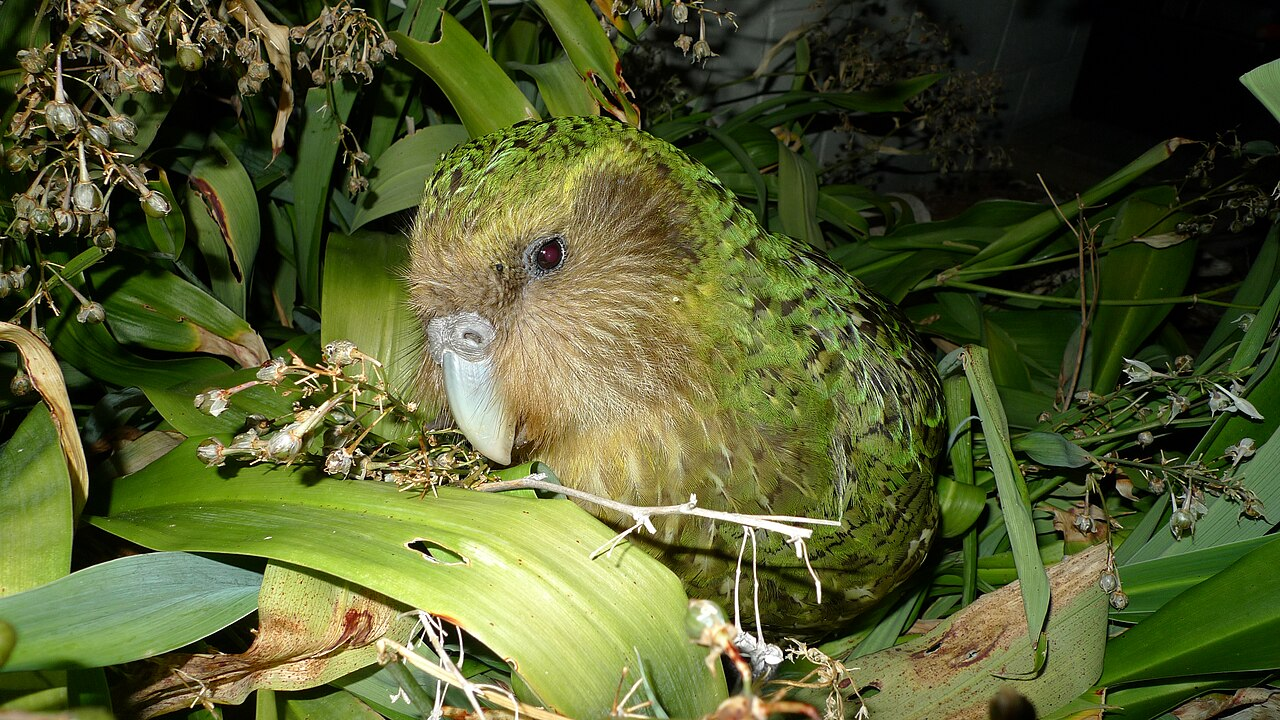
\includegraphics[width=0.46\linewidth]{images/book5/kakapo-sirocco.jpg}\hspace{0.04\linewidth}
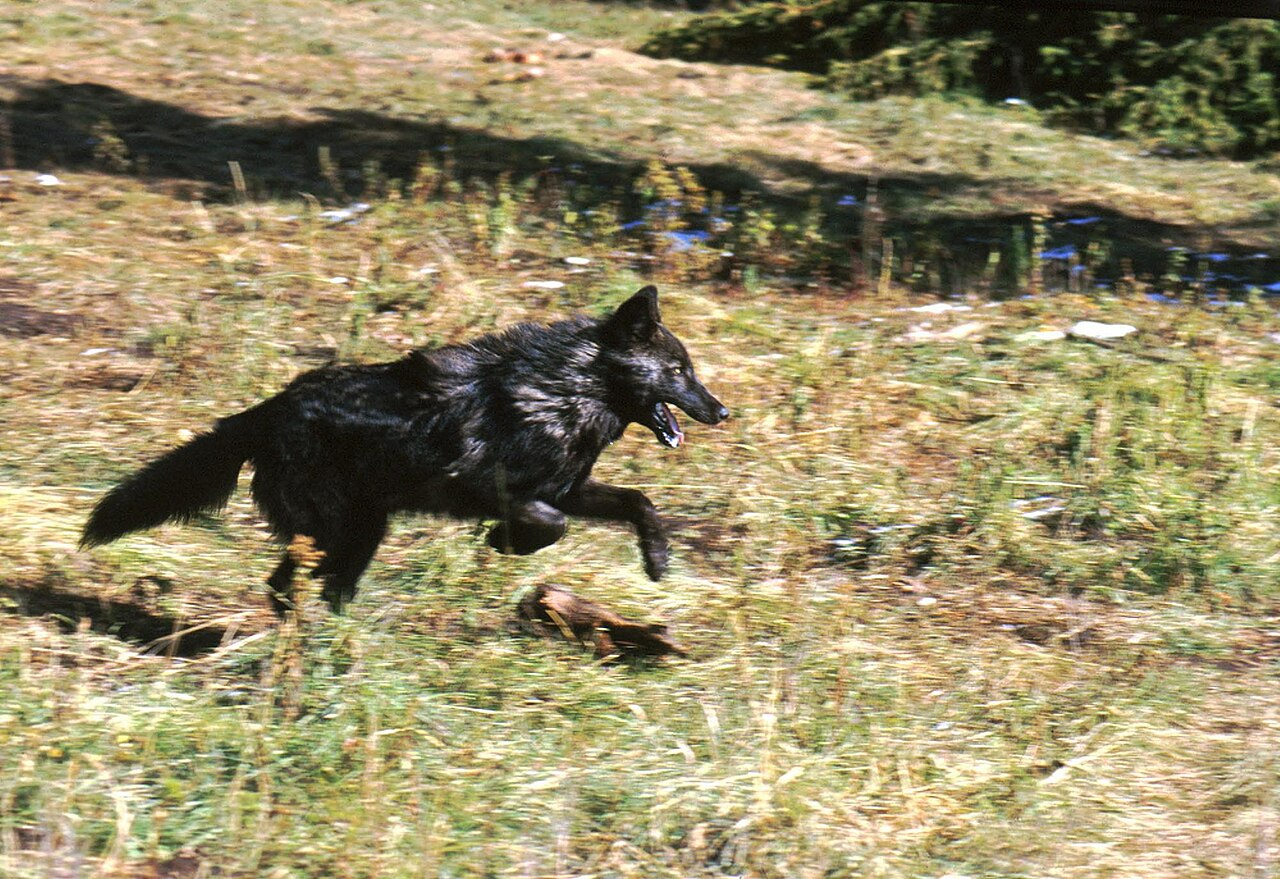
\includegraphics[width=0.46\linewidth]{images/book5/yellowstone-wolves-1996.jpg}

{\small À esquerda: Sirocco, um kakapo --- um dos cinquenta e um
sobreviventes de 1995, hoje um de uns duzentos e cinquenta, cada um
nomeado e monitorado em ilhas livres de predadores (fotografia:
Department of Conservation, Nova Zelândia, CC BY 2.0). À direita: lobos
em Yellowstone em 1996, o primeiro inverno após sua \omterm{def:b3:conservation-biology:tools}{reintrodução}
(fotografia: National Park Service, domínio público).}
\end{omfigure}

\begin{example}[Três recuperações]\label{ex:b3:conservation-biology:recoveries}
O kakapo: cinquenta e uma aves em 1995, todas levadas para ilhas limpas
de predadores; cada ave carrega um transmissor, cada ninho é vigiado por
câmera, os filhotes são criados à mão quando uma mãe falha, os machos são
alimentados para entrarem em condição reprodutiva nos anos em que as
árvores de rimu frutificam, e o pedigree é manejado para manter na
população os genes raros do último macho de Fiordland; o genoma de cada
kakapo foi sequenciado. São duzentos e cinquenta agora, e um $N_{e}$ que
os genomas põem perto de cem. O grou-americano: quinze aves em 1941, um
único bando migratório, criado em cativeiro a partir de ovos retirados de
ninhos silvestres, ensinado a novas rotas de migração atrás de aviões
ultraleves, e hoje uns oitocentos. A baleia-jubarte: caçada até uns
poucos milhares, protegida em 1966, e hoje além de cem mil, um aumento
perto de \qty{8}{\%} ao ano que mostra o que um animal longevo faz quando
a única causa de seu declínio é removida. Cada recuperação custou dezenas
de milhões e décadas; a aritmética do capítulo diz por que o esforço teve
de ser gasto antes que os números chegassem ao vórtice, e por que ele
saiu mais barato que qualquer resgate posterior.
\end{example}

\begin{omfigure}
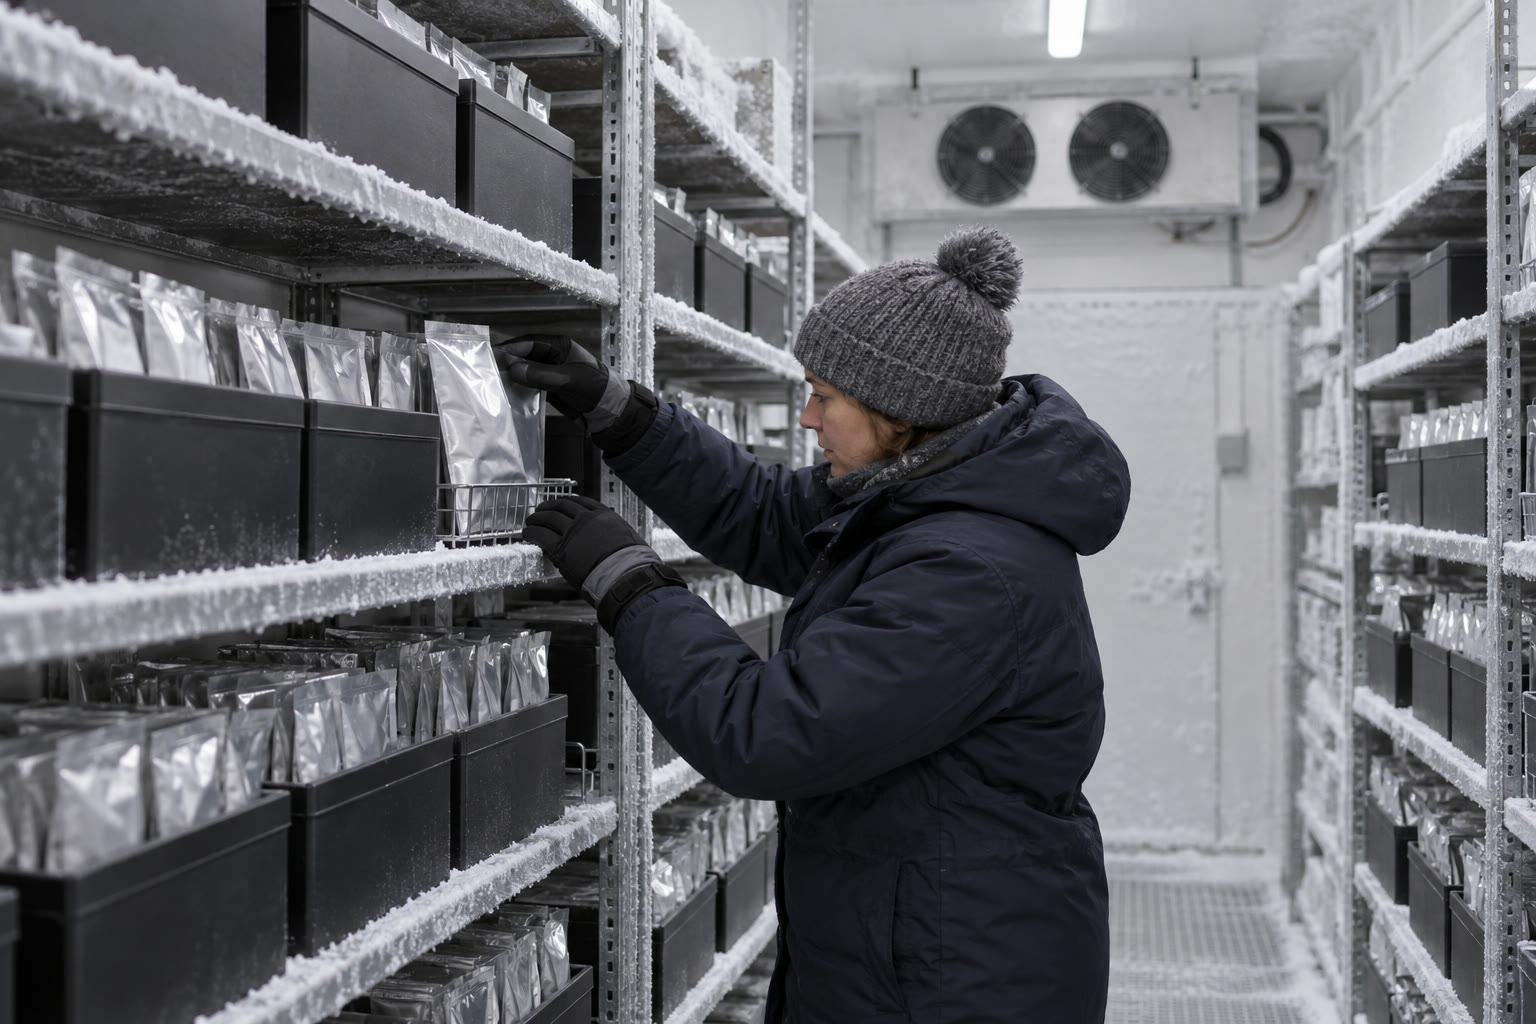
\includegraphics[width=0.56\linewidth]{images/book5/ai/b5-27-seed-vault.jpg}

{\small Um cofre de sementes no permafrost: duplicatas de um milhão de
acessos de plantas cultivadas e silvestres, mantidas a
\qty{-18}{\celsius} contra a perda das coleções de onde vieram --- a
conservação como seguro, na escala do genoma de uma espécie.}
\end{omfigure}

\begin{remark}[A aritmética de manter]\label{rem:b3:conservation-biology:remark}
Cada capítulo deste curso terminou num número, e este termina em vários:
um tamanho efetivo, um \omterm{thm:b3:conservation-biology:ne}{coeficiente de endogamia} subindo $1/2N_{e}$ por
geração, um expoente $z$ que converte hectares perdidos em espécies
perdidas, uma probabilidade de extinção ao longo de um século. Eles são
grosseiros --- o censo é incerto, a variância é adivinhada, o modelo é uma
caricatura --- e são o que transforma um sentimento a respeito de aves
que somem numa decisão sobre que cinquenta hectares comprar e que oito
animais mudar de lugar. A biologia é a mesma biologia do resto do livro:
deriva, seleção, demografia, comportamento, a dependência de uma
população de seu hábitat e de um hábitat de suas populações. O que há de
novo é apenas a urgência, e o fato de que o experimento está sendo feito
uma única vez, sem controle, sobre as espécies que restam.
\end{remark}

\section{Exercícios}

\begin{exercise}[$\star$]\label{exo:b3:conservation-biology:1}
Defina \omterm{def:b3:conservation-biology:small}{estocasticidade demográfica}, \omterm{def:b3:conservation-biology:small}{estocasticidade ambiental} e \omterm{def:b3:conservation-biology:small}{efeito
Allee}, e dê um exemplo de cada um tirado do capítulo.
\end{exercise}

\begin{exercise}[$\star$]\label{exo:b3:conservation-biology:2}
O que é o \omterm{thm:b3:conservation-biology:ne}{tamanho efetivo da população}, e nomeie três características de
uma população real que o tornam menor que o censo.
\end{exercise}

\begin{exercise}[$\star$]\label{exo:b3:conservation-biology:3}
Enuncie a lei espécies--área. Se $z = 0.25$, que fração das espécies um
hábitat mantém depois de perder metade de sua área? E nove décimos? E
noventa e nove centésimos?
\end{exercise}

\begin{exercise}[$\star$]\label{exo:b3:conservation-biology:4}
Explique a regra 50/500 e contra o que cada número protege.
\end{exercise}

\begin{exercise}[$\star\star$]\label{exo:b3:conservation-biology:5}
Um bando de 200 elefantes-marinhos tem 8 machos e 120 fêmeas
reprodutores. Calcule $N_{e}$ e a perda de heterozigosidade por geração.
Quantas gerações para perder um quarto dela?
\end{exercise}

\begin{exercise}[$\star\star$]\label{exo:b3:conservation-biology:6}
Uma população contou 1000, 1000, 20, 1000, 1000 em cinco gerações
sucessivas. Calcule $N_{e}$ no intervalo e a heterozigosidade retida, e
compare com um valor constante de 1000.
\end{exercise}

\begin{exercise}[$\star\star$]\label{exo:b3:conservation-biology:7}
Vinte e cinco panteras-da-flórida com $N_{e} \approx 10$: endogamia
acumulada em 5 gerações? Se a aptidão cai \qty{5}{\%} a cada \qty{10}{\%}
de $F$, de quanto ela caiu? O que acrescentar oito fêmeas não aparentadas
faz com $F$ na geração seguinte?
\end{exercise}

\begin{exercise}[$\star\star$]\label{exo:b3:conservation-biology:8}
Yellowstone: 31 lobos soltos em 1995--96, cerca de 100 no parque em 2003.
Estime $r$; quantos haveria em 2020 se o crescimento tivesse continuado,
e por que ele não continuou?
\end{exercise}

\begin{exercise}[$\star\star$]\label{exo:b3:conservation-biology:9}
Classifique pelos critérios da IUCN vistos no capítulo: (a) uma rã cuja
população caiu \qty{60}{\%} em dez anos; (b) uma planta de 180 indivíduos
maduros; (c) um peixe cuja área de distribuição é de \qty{3000}{km^2};
(d) uma ave de \num{30000} indivíduos declinando \qty{10}{\%} por
década.
\end{exercise}

\begin{exercise}[$\star\star\star$]\label{exo:b3:conservation-biology:10}
Uma população de $N$ casais, cada um produzindo, com probabilidade $1/2$,
dois descendentes sobreviventes e, caso contrário, nenhum
(\omterm{def:b3:conservation-biology:small}{estocasticidade demográfica}). Calcule a probabilidade de que toda a
população falhe em uma geração para $N = 2$, $5$, $10$, $20$, e comente
como o risco demográfico escala com $N$.
\end{exercise}

\begin{exercise}[$\star\star\star$]\label{exo:b3:conservation-biology:11}
A lei espécies--área com $z = 0.25$, e uma floresta cortada em 10
fragmentos isolados iguais. Compare as espécies esperadas num fragmento
com as de um décimo da original, e argumente por que o total entre os
fragmentos não é simplesmente o original --- o que determina se os
fragmentos juntos abrigam mais ou menos espécies que o todo abrigava?
\end{exercise}

\begin{exercise}[$\star\star\star$]\label{exo:b3:conservation-biology:12}
Por que acrescentar uns poucos migrantes por geração ($m N_{e} \approx 1$) praticamente interrompe a perda de variação numa população pequena, e
o que isso custa em adaptação local? Use o equilíbrio entre a deriva,
$1/2N_{e}$, e a fração de alelos substituídos por migrantes, $m$, para
argumentar.
\end{exercise}

\section{Problema: Cinquenta e Quinhentos}

\begin{problem}[{Problema de fim de semana --- um programa de recuperação
em números: o tamanho efetivo de uma população resgatada de papagaios e
sua endogamia, um resgate genético, as espécies que uma floresta em
encolhimento manterá, o crescimento de lobos reintroduzidos, e as
categorias e os custos, terminando em $N_{e}$, na endogamia após dez
gerações e na fração de espécies mantida}]
\label{pb:b3:conservation-biology:1}
Dados: uma população de papagaios de 60 adultos, 20 machos e 40 fêmeas,
todos reprodutores; tempo de geração \qty{10}{yr}. História da população
nas últimas cinco gerações: 500, 100, 60, 51, 60. Depressão endogâmica: a
aptidão cai \qty{6}{\%} a cada \qty{0.1}{} de $F$. Resgate: 10 aves não
aparentadas acrescentadas às 60. Floresta: \qty{2000}{km^2} reduzidos a
\qty{300}{km^2}, $z = 0.25$; espécies hoje, 180. Lobos: 31 soltos, 100
após 8 anos, capacidade de suporte no parque de cerca de 120. Custo:
quatro milhões de dólares por ano para os papagaios.

\medskip
\noindent\textbf{Parte I --- Tamanho efetivo.}
\begin{enumerate}
  \item $N_{e}$ a partir da \omterm{thm:b3:conservation-biology:ne}{razão sexual} dos 60 atuais. Compare com o
        censo.
  \item $N_{e}$ como \omterm{thm:b3:conservation-biology:ne}{média harmônica} ao longo das cinco gerações da
        história. Que geração domina?
  \item Endogamia acumulada ao longo dessas cinco gerações, usando o
        $N_{e}$ da \omterm{thm:b3:conservation-biology:ne}{média harmônica} (fórmula exata e aproximação linear).
  \item Aptidão perdida por essa endogamia.
  \item Heterozigosidade retida após as cinco gerações, como fração da
        original.
  \item Se a população for mantida agora em 60 com a \omterm{thm:b3:conservation-biology:ne}{razão sexual} atual,
        que $F$ ela alcançará em mais dez gerações, e que perda de
        aptidão? Quantos anos são?
\end{enumerate}

\medskip
\noindent\textbf{Parte II --- Resgate.}
\begin{enumerate}[resume]
  \item Dez aves não aparentadas se juntam às 60. A fração de alelos da
        geração seguinte vinda dos recém-chegados é de cerca de $10/70$;
        o \omterm{thm:b3:conservation-biology:ne}{coeficiente de endogamia} dos filhotes com um progenitor nativo
        e um recém-chegado é $0$. Estime o $F$ médio da população na
        geração seguinte se o acasalamento for aleatório.
  \item Explique por que $F$ cai de imediato mas a heterozigosidade só
        sobe à medida que os alelos dos migrantes se espalham, e por que
        um segundo resgate pode ser necessário.
  \item Para alcançar $N_{e} = 500$ com \omterm{thm:b3:conservation-biology:ne}{razão sexual} igual, quantos
        adultos são necessários? A $r = \qty{0.05}{yr^{-1}}$ a partir de
        70 aves, quantos anos?
  \item O programa retira ovos de mães ruins para criação à mão, elevando
        o número médio de filhotes emplumados por casal mas igualando os
        tamanhos das famílias. Por que igualar os tamanhos das famílias
        \emph{eleva} $N_{e}$ acima do censo (rumo a $2N$)?
  \item O último macho de uma linhagem meridional distinta é estéril na
        natureza. Proponha duas intervenções e seus custos para o
        patrimônio genético.
  \item A quatro milhões de dólares por ano ao longo dos 40 anos até
        alcançar $N_{e} = 500$, custo total e custo por ave acrescentada.
        Isso é caro? Comparado com o quê?
\end{enumerate}

\medskip
\noindent\textbf{Parte III --- Floresta.}
\begin{enumerate}[resume]
  \item Fração das espécies que a floresta manterá com \qty{300}{km^2};
        número esperado de espécies e a dívida de extinção (espécies
        presentes hoje que serão perdidas).
  \item Se, em vez disso, os \qty{300}{km^2} fossem três fragmentos
        isolados de \qty{100}{km^2}, espécies por fragmento; total se os
        fragmentos abrigassem espécies inteiramente diferentes; total se
        abrigassem as mesmas. O que decide?
  \item Um corredor de \qty{20}{km^2} une os três fragmentos. Trate-os
        como uma área única de \qty{320}{km^2}: espécies esperadas.
        Compare com o caso de espécies idênticas da questão~14.
  \item O maior predador da floresta precisa de \qty{50}{km^2} por casal
        e de um $N_{e}$ de 50 para persistir. Os \qty{300}{km^2} inteiros
        conseguem abrigá-lo? E um fragmento? O que isso diz sobre a área
        contra o número de espécies como critério?
  \item Estime quanto tempo a dívida de extinção leva para ser paga se as
        espécies perdidas tiverem populações declinando \qty{3}{\%} ao
        ano de 200 até um limiar de \omterm{met:b3:conservation-biology:pva}{quase extinção} de 10.
  \item Por que a lei espécies--área subestima a perda quando a
        fragmentação acrescenta \omterm{prop:b3:conservation-biology:area}{efeitos de borda}, e a superestima quando
        a terra do entorno é em parte utilizável?
\end{enumerate}

\medskip
\noindent\textbf{Parte IV --- Lobos e listas.}
\begin{enumerate}[resume]
  \item Lobos: $r$ de $31 \to 100$ em 8 anos, e o tempo de duplicação.
  \item Crescimento logístico rumo a $K = 120$: população após 8 anos sob
        crescimento logístico em vez de exponencial, partindo de 31 com o
        $r$ da questão~19 (use $N(t) = K/[1 + (K/N_{0} -
        1)\mathrm{e}^{-rt}]$). Qual se ajusta melhor aos 100 observados, e
        o que isso diz sobre a dependência da densidade nos primeiros
        anos?
  \item Os wapitis eram \num{17000} em 1995 e \num{4000} em 2015. Taxa
        média anual de declínio. Quanto dela lobos que comem \num{20}
        wapitis cada por ano conseguem explicar, com 100 lobos?
  \item Classifique o papagaio (60 indivíduos maduros) e o predador da
        floresta antes do resgate pelos critérios da IUCN.
  \item Pombo-passageiro: cinco bilhões em 1800, extinto em 1914. Se o
        declínio foi exponencial de 1870, quando ainda eram bilhões, até
        uma ave em 1914, que taxa anual isso implica? Por que o \omterm{def:b3:conservation-biology:small}{efeito
        Allee} torna as últimas décadas mais rápidas que a exponencial?
  \item Explique num parágrafo por que uma AVP teria dito que o
        pombo-passageiro estava seguro em 1850, e o que ela teria
        deixado passar.
  \item Resuma: o $N_{e}$ atual (questão~1), o $F$ após mais dez gerações
        com 60 (questão~6) e a fração de espécies que a floresta encolhida
        mantém (questão~13).
\end{enumerate}
\end{problem}
